\section{User interface}\label{sc:userinterface}
% intro intro

\begin{figure}[H]
    \centering
    \frame{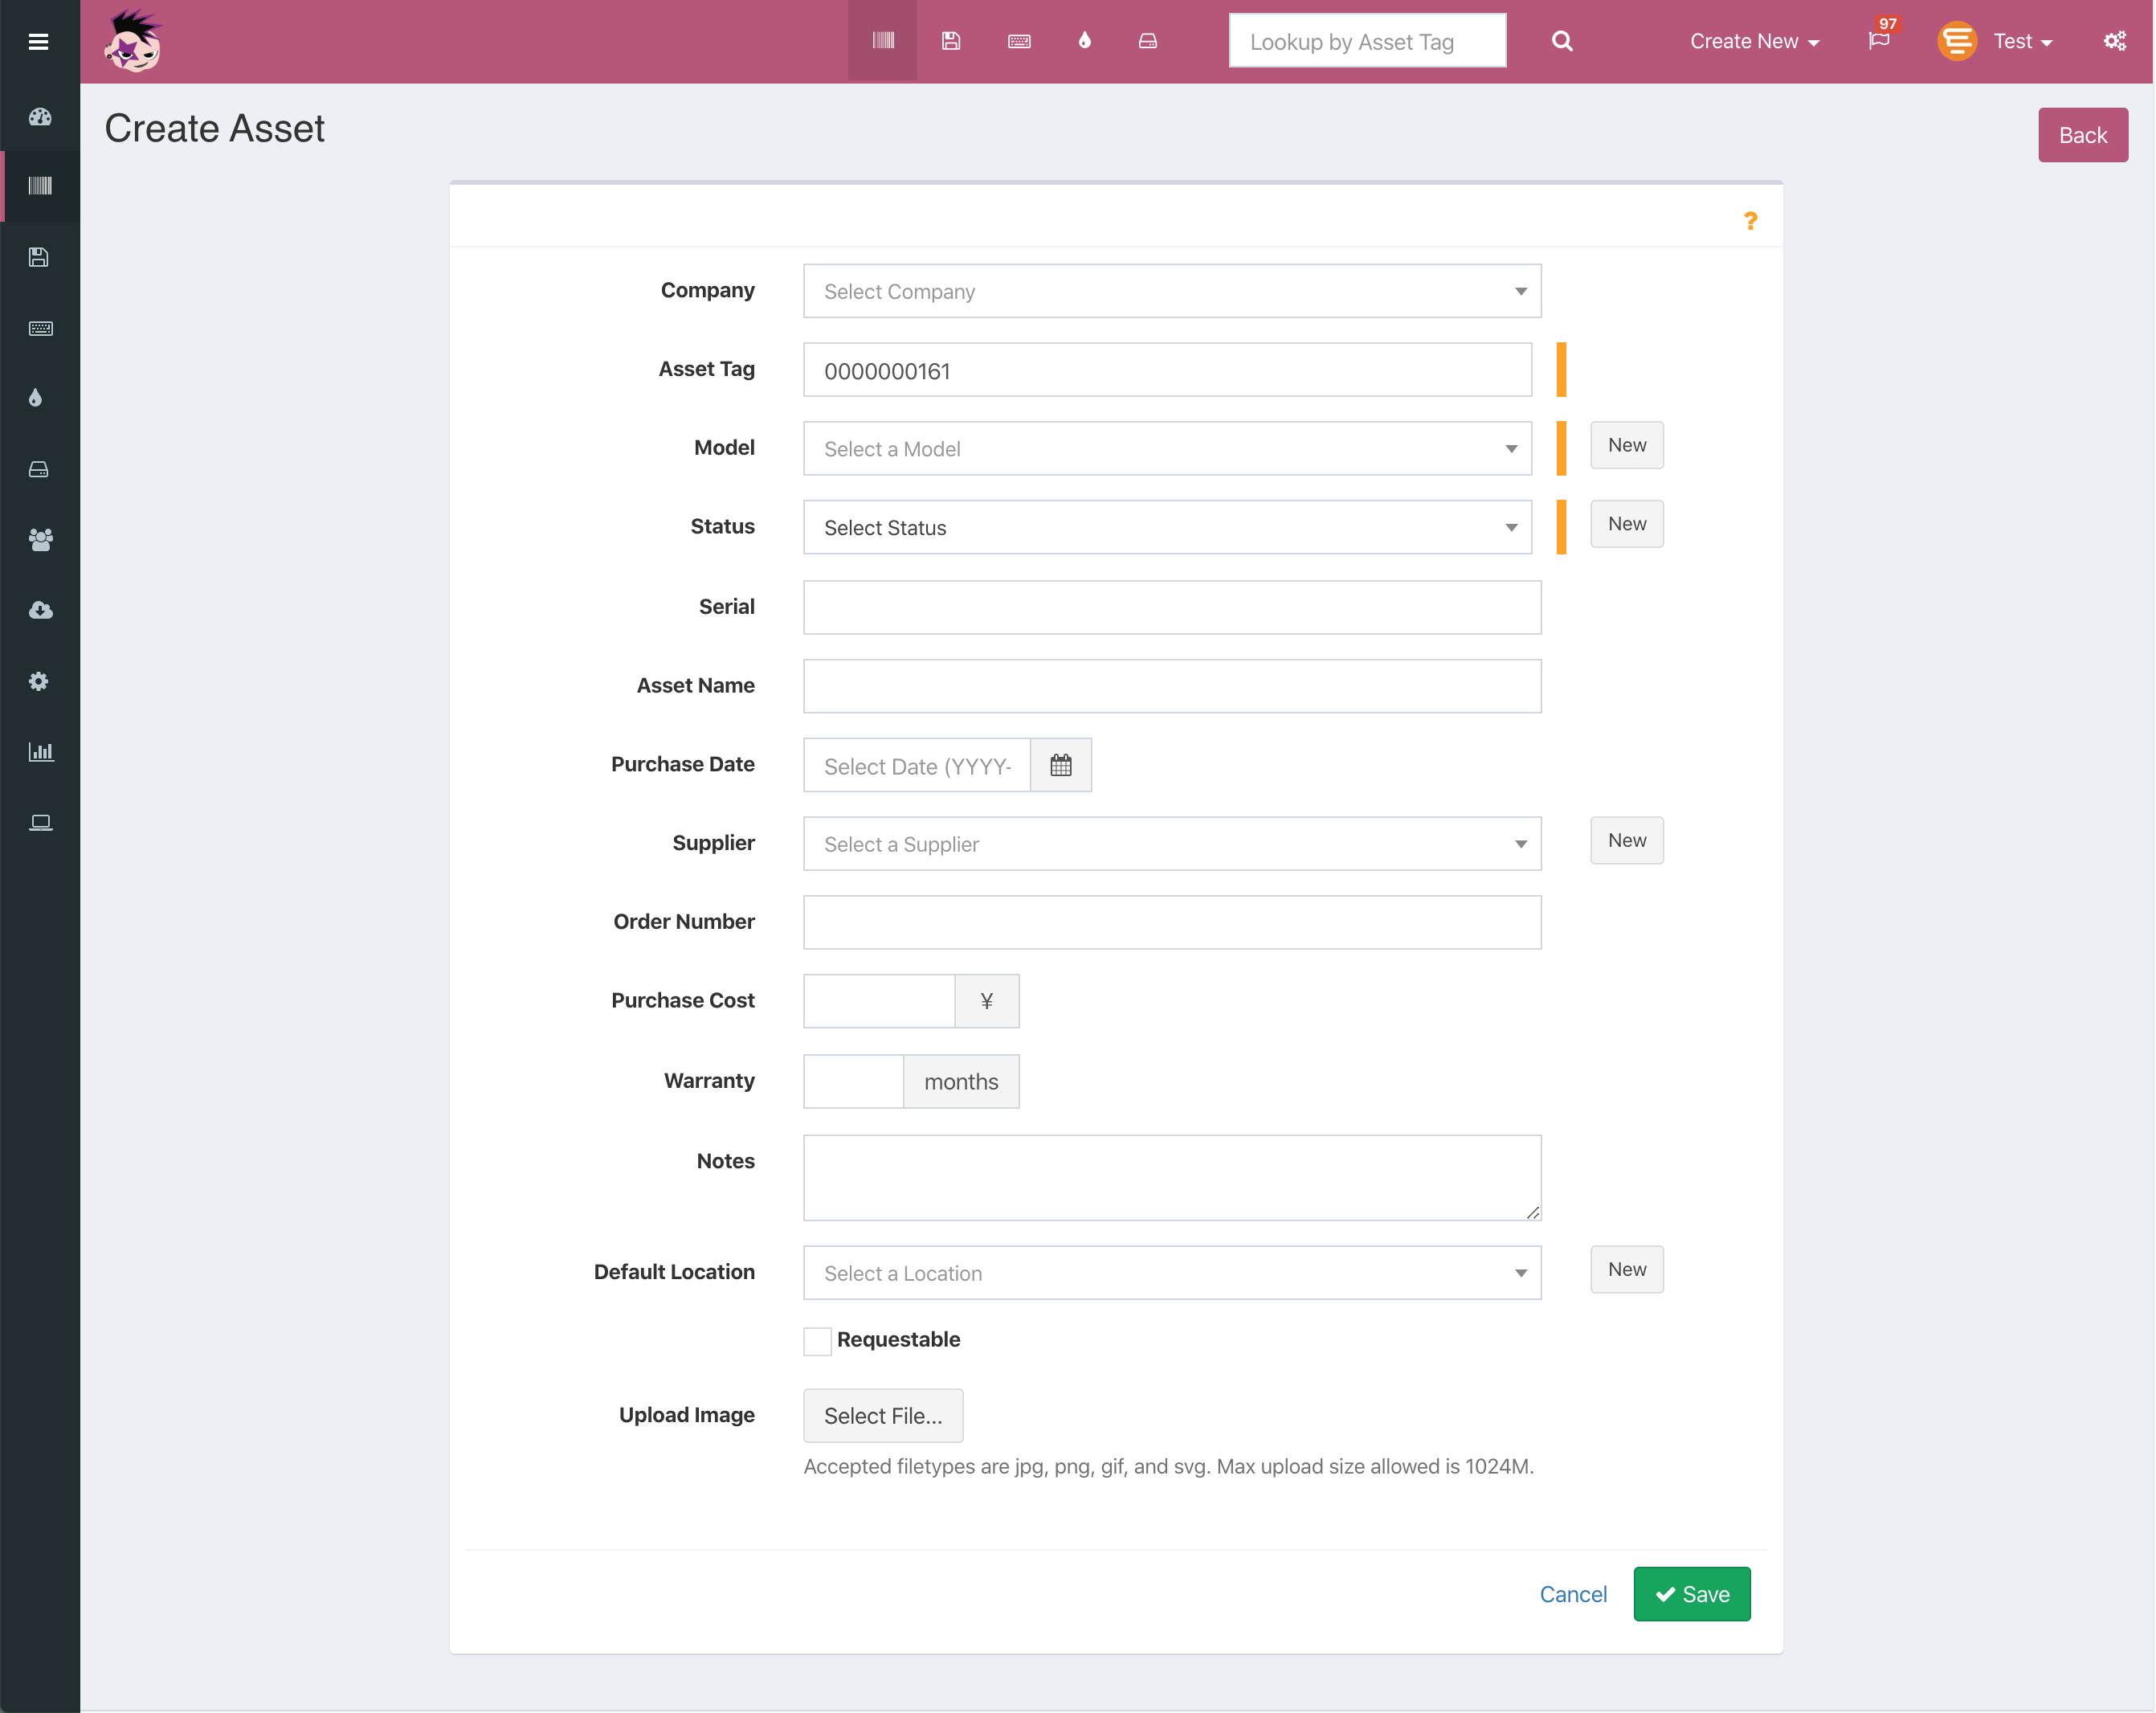
\includegraphics[width=0.9\textwidth]{figures/other-systems/snipeitapp-create-asset-ui-screenshot.png}}
    \caption{Caption}
    \label{fig:too}
\end{figure}


The user interface is following the KISS-principle (Keep It Simple Stupid) and therefore only contains the utmost required interface-elements. As mentioned in \autoref{ch:introduction} and \autoref{ch:problemdefinition} our client needs an easier process of maintaining assets compared to existing solutions on the market. Existing solutions often present the user with a number of fields depending on the category an asset belongs to. This often result in empty and unnecessary fields that are never used. Our approach is based on fields dynamically appearing based on tags added to an asset.

\begin{figure}[H]
    \centering
    \frame{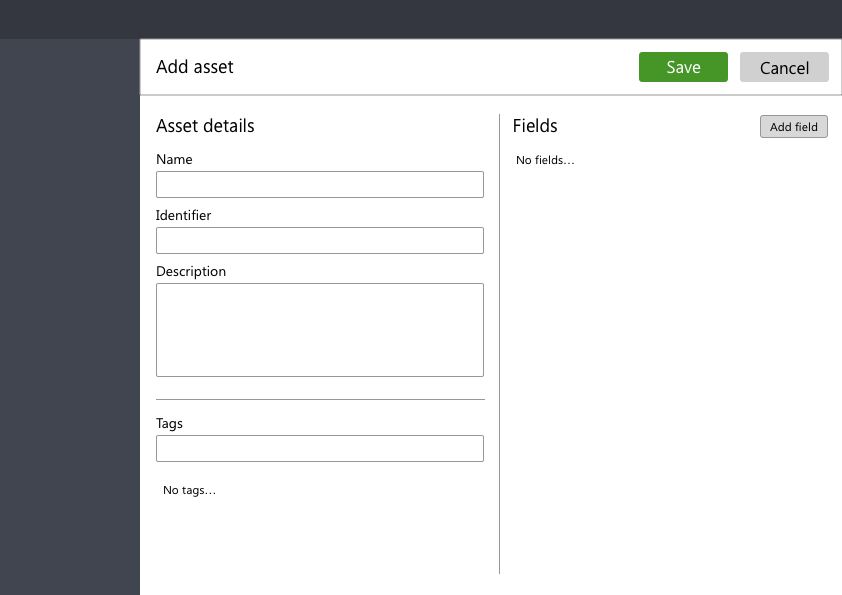
\includegraphics[width=0.9\textwidth]{figures/wireframes/add-asset-no-tags.png}}
    \caption{The process of creating a new asset, at this point no tags or custom fields were added, resulting in no fields beside base fields.}
    \label{fig:add-asset-no-tags}
\end{figure}

\begin{figure}[H]
    \centering
    \frame{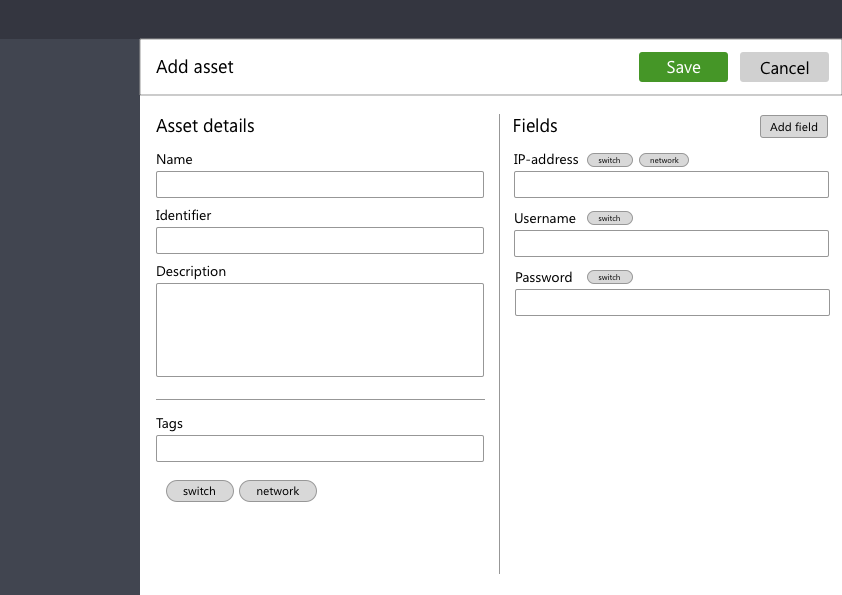
\includegraphics[width=0.9\textwidth]{figures/wireframes/add-asset-with-tags.png}}
    \caption{User interface state chart diagram for searching for an asset}
    \label{fig:add_asset_with_tags}
\end{figure}


\subsection{Employee}
Employees have access to the application and are capable of performing basic operations within the system.

\textbf{Splashscreen:} the first screen visible to the user at application startup 

% Dash / overview page
% Assets list page
% Asset view
% Add comments to asset
% Edit/remove own assets
% Menues?

\subsection{Admin}
Admins are able to do everything an Employee can but their enhanced access make them able to manage system content.

% Add/edit/delete departments
% Add/edit/delete assets
% Add/edit/delete tags
% Add/edit/delete all comments
% Read logs
% Export reports
% Import user data from third-part // Allowing employees access to the system
% 